\documentclass{standalone}

\usepackage[english]{babel}

% to define font size

\usepackage{ulem}
\usepackage{moresize}
\usepackage{anyfontsize}

% to use colors

\usepackage[dvipsnames]{xcolor}
\usepackage{MnSymbol}

% to use tikz and its libraries

\usepackage{tikz-timing}
\usepackage{tikz}

\usetikzlibrary{backgrounds}
\usetikzlibrary{positioning, calc, arrows, shapes, automata, petri, patterns, decorations.markings}
\usetikzlibrary{decorations.pathreplacing}

% to use tikzmark, to place and refer to marks outside the current figure

\tikzset{every picture/.style={remember picture}}

% styles for transitions

\tikzset{transition/.append style={fill=black!20, thick}}
\tikzset{transition/.append style={fill=black!20, thick}}

% styles for test and inhib arcs.

\tikzstyle{test}=[pre, *-]
\tikzstyle{inhib}=[pre, o-]

\usepackage{circuitikzgit}
\ctikzset{
  logic ports=ieee,
}

% Arrow positioning in a path

\tikzset{->-/.style={decoration={
  markings,
  mark=at position #1 with {\arrow{>}}},postaction={decorate}}}

\tikzset{-<-/.style={decoration={
  markings,
  mark=at position #1 with {\arrow{<}}},postaction={decorate}}}

% shift values

\newcommand{\outportshift}{0mm}
\newcommand{\outportidpshift}{0mm}

%%%%%%%%%%%%%%%%%%%%%%%%%%%%%%%%%%%%%%%%%%%%%%%%%%
%                  BEGIN DOCUMENT                %
%%%%%%%%%%%%%%%%%%%%%%%%%%%%%%%%%%%%%%%%%%%%%%%%%%

\begin{document}

\begin{circuitikz}

  \ctikzset{multipoles/dipchip/width=1.5}
  \ctikzset{multipoles/dipchip/pin spacing=.33}

  \node (pn) {
    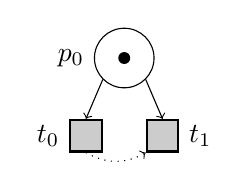
\begin{tikzpicture}

      % PLACES AND TRANSITIONS

      \node[place, tokens=1] (p0)  {};
      \node[transition, anchor=north east] (t0) at ($(p0.south west)-(0,.5)$) {};
      \node[transition, anchor=north west] (t1) at ($(p0.south east)-(0,.5)$) {};
      
      % LABELS

      \node[anchor=east] (tzLabel) at ($(t0.west)$) {$t_0$};
      \node[anchor=west] (tzLabel) at ($(t1.east)$) {$t_1$};
      \node[anchor=east] (pzLabel) at ($(p0.west)$) {$p_0$};
      
      % ARCS
      \draw[->] ($(p0.south west)$) -- ($(t0.north)$);
      \draw[->] ($(p0.south east)$) -- ($(t1.north)$);
      \draw ($(t0.south)$) edge[->, dotted, bend right] ($(t1.south west)$);
      
    \end{tikzpicture}
  };

  % PDI idp0
  
  \draw       
  node [dipchip, num pins=4, hide numbers,
  no topmark, external pins width=0]
  (idp0) at ($(pn.east)+(2.5,0)$) {};

  \node[anchor=south] at ($(idp0.north)$) {$\gamma(p_0)$};

  \draw ($(idp0.bpin 1)$)
  node [anchor=west, font=\ssmall]  {\tt otf(i)};
  
  \draw ($(idp0.bpin 2)$)
  node [anchor=west, font=\ssmall] {\tt otf(j)};

  \draw ($(idp0.bpin 4)$)
  node [anchor=east, font=\ssmall]  {$id_{out}\mathtt{(i)}$};

  \draw ($(idp0.bpin 3)$)
  node [anchor=east, font=\ssmall]  {$id_{out}\mathtt{(j)}$};
  
  % TDI idt0
  
  \draw       
  node [dipchip, num pins=2, hide numbers,
  no topmark, external pins width=0]
  (idt0) at ($(idp0.east)+(2,1)$) {};

  \node[anchor=south] at ($(idt0.north)$) {$\gamma(t_0)$};
  
  \draw ($(idt0.bpin 1)$)
  node [anchor=west, font=\ssmall]  {$name_{t_0}$};

  \draw ($(idt0.east)$)
  node [anchor=east, font=\ssmall]  {\tt f};

  % TDI idt1
  
  \draw       
  node [dipchip, num pins=2, hide numbers,
  no topmark, external pins width=0]
  (idt1) at ($(idp0.east)+(2,-1)$) {};

  \node[anchor=south] at ($(idt1.north)$) {$\gamma(t_1)$};
  
  \draw ($(idt1.bpin 1)$)
  node [anchor=west, font=\ssmall]  {$name_{t_1}$};

  \draw ($(idt1.east)$)
  node [anchor=east, font=\ssmall]  {\tt f};

  % INTERCONNECTIONS

  \draw[red,->-=.5] ($(idp0.bpin 4)$) --++(.3,0) |- ($(idt0.bpin 1)$);
  \draw[red,->-=.5] ($(idp0.bpin 3)$) --++(.3,0) |- ($(idt1.bpin 1)$);
  \draw[red,-<-=.5] ($(idp0.bpin 1)$) -|++ (-.3, 1.7) -| ($(idt0.east)+(.3,0)$) -- (idt0.east);
  \draw[red,-<-=.5] ($(idp0.bpin 2)$) -|++ (-.3, -1.2) -| ($(idt1.east)+(.3,0)$) -- (idt1.east);

  
  % TRANSLATION ARROW
  
  \node at ($(pn.east)!.3!(idp0.west)$) {\Huge$\rightarrow$};

  % I < J
  \node[red] at ($(idp0.east)!.5!(idt1.west)-(0,1.5)$) {\Large $i<j$};
  
  
\end{circuitikz}


\end{document}
%%% Local Variables:
%%% mode: latex
%%% TeX-master: t
%%% End:
